\chapter{Réalisation}

\section{Introduction}
    Dans ce chapitre nous allons présenter l'environnement de développement de l'application.\\

    Nous commencerons par les techniques utilisés puis passerons vers les bibliothèques et les frameworks qui ont aidé dans cette réalisation. Par la suite, nous présenterons les outils utilisés tout le long du processus de création.\\

    Finalement, nous présenterons quelles ques interfaces de l'application.\\

\section{Présentation des technologies utilisées}
    Le but du projet est la création d'une application full-stack web. pour cela, plusieurs outils peuvent être utilisés, parmi ces outils, nous avons choisi \acs{PERN} qui est une pile de technologies conçues justement pour la création d'un environnement de développement full-stack web. \acs{PERN}, par ses initiales, se compose de PostgreSQL, ExpressJS, React et Node.js.\\

    \acs{PERN} est un substitué de \acs{MERN}, qui est lui-même composer de MongoDB, ExpressJS, React et Node.js. Comme \acs{MERN}, \acs{PERN} donne la possibilité de créer des applications web full-stack avec des opérations \acs{CRUD} (Create, Read, Update, Delete). Mais \acs{PERN} utilise PostgreSQL au lieu de MongoDB est nous offre un grand support pour les fonctionnalités \acs{NoSQL}, avec une forte conformité aux normes et prend en compte les transactions.\\

    \subsection{PostgreSQL}
    \begin{figure}[H]
        \centering
        
\includegraphics[scale=0.2]{ACR/postgresql.png}
        \caption{Logo PostgreSQL}
    \end{figure}
    
    PostgreSQL\cite{postgres} est système de gestion de base de données relationnel orienté objet puissant et open-source, qui utilise \acs{SQL} et prend en charge en toute sécurité les charges de travil complexes en regroupant plusieurs fonctionnalités qui donnent priorité à l'extensibilité et la conformité.\\

    L'origine de PostgreSQL remonte a la base de données Ingres développer à l'université de la Californie de Berkley par Michael Stonebraker. Au années 1986, son créateur a repris le projet de zero est a décidé de le nommée POSTGRES, comme pour dire post-ingres. Ce n'est qu'en 1995 que son créateur à décidé d'ajouter les fonctionnalitées \acs{SQL} est a été renommée Postgre95, et ce fut qu'à la fin des années 1996 qu'il a été renommée en PostgreSQL.\\
    
    Avec plus de 30 années de développement, PostgreSQL a gagné une forte réputation grace a son architecture, sa robustesse, son extensibilité et le dévouement des contributeurs de la communauté open-source.\\

    \subsection{ExpressJS}
    \begin{figure}[H]
        \centering
        
\includegraphics[scale=0.16]{ACR/ExpressJS-logo.png}
        \caption{Logo ExpressJS}
    \end{figure}
    
    ExpressJS\cite{expressjs} est un framework Node.js qui fournit des fonctions puissantes pour les applications web et mobiles. Il est très simple, très léger et très flexible. Il apporte très peu de couverture et maintient le meilleur côté et une exécution rapide.\\

    En vue de son côté open source et facile d'utilisation, ExpressJS connaît une grande notoriété et possède grace aux contributeurs une grande bibliothèque de modules prêt à l'employer. ExpressJS améliore Node.js, de façons à construire rapidement, facilement et efficacement les APIs les plus complexes.\\ 

    \subsection{React}
    \begin{figure}[H]
        \centering
        
\includegraphics[scale=0.16]{ACR/react.png}
        \caption{Logo REACT}
    \end{figure}

    React\cite{react} est une bibliothèque JavaScript conçue pour créer des interfaces utilisateur interactives et rapides pour les applications Web et mobiles. React a été créé par Jordan Walke, ingénieur logiciel chez Facebook.\\
    
    React s'agit d'une bibliothèque frontend open source, basée sur des composants réutilisables, qui n'est responsable que de la couche de vue (View) des application basé sur l'architecture Model View Controller (\acs{MVC}). L'une des forces de React est la modification de données sans rechargement de page. Cette spécialisation permet à React d'être combiné avec plusieurs bibliothèques ou frameworks pour former une application fullstack.\\

    \subsection{Node.js}
    \begin{figure}[H]
        \centering
        
\includegraphics[scale=0.1]{ACR/nodejs-logo.png}
        \caption{Logo Node.js}
    \end{figure}

    Node.js\cite{nodejs} est un environnement d'exécution JavaScript open source et multiplateforme qui peut exécuter du code JavaScript en dehors du navigateur Web. Node.js est un framework Web léger et populaire, adapté aux débutants, mais aussi utilisé dans de nombreuses grandes entreprises telles que Netflix et Uber l'utilisent.\\
    
    Node.js est un framework Web très approprié pour les débutants, il permet de pouvoir facilement démarrer la construction back-end. Il nous permet d'utiliser JavaScript n'importe où et sur n'importe quel navigateur, y compris MacOS, Linux et Windows. Quand nous disons omniprésent, nous faisons référence au front-end, au middleware et au back-end. Par conséquent, Node.js fait partie de certaines piles de développement Web très populaires, telles que la pile \acs{MERN}, la pile \acs{MEVN} et la pile \acs{MEAN}.\\

\section{Bibliothèques et Framework utilisés}
    Le but des bibliothèques et des frameworks est de nous faciliter et d'acculer le processus de développement. Celle-ci nous apportent des fonctions déjà créées et ne nous restent plus qu'a les utilisé.\\

    Voici donc qu'elles unes de ces bibliothèques et frameworks:\\

    \subsection{Axios}
    \begin{figure}[H]
        \centering
        
\includegraphics[scale=1]{ACR/axios-logo.png}
        \caption{Logo Axios}
    \end{figure}

    Axios\cite{axios} est un client HTTP basé sur des promesses qui peut s'exécuter dans un navigateur et un environnement Node.js. Il fournit une API pour traiter les requêtes XMLHttpRequests et l'interface http du nœud. De plus, il utilise également la requête d'emballage polyfill de la nouvelle syntaxe de promesse d'ES6.\\
    
    Presque tous les projets dynamiques que vous créez doivent interagir avec l'API RESTFUL à un moment donné, et l'utilisation d'Axios est un moyen simple de le faire. La première version d'Axios est sortie il y a environ 4 ans, et son code open source est disponible sur GitHub. Axios compte plusieurs contributeurs qui ont contribué à chaque version d'Axios.\\

    \subsection{Redux}
    \begin{figure}[H]
        \centering
        
\includegraphics[scale=0.2]{ACR/redux-logo.png}
        \caption{Logo Redux}
    \end{figure}

    Redux\cite{redux} est une bibliothèque JavaScript open source pour la gestion des "state" de l'application. Redux est généralement utilisé avec des bibliothèques telles que Angular ou React pour créer des interfaces utilisateur. Il a été créé par Andrew Clark et Dan Abramov.\\
    
    Lorsque la taille de l'application devient très importante, il devient difficile de gérer le state de chaque composant de l'application. Il permet de mettre à jour et de maintenir le state de chaque composant de l'application.\\

    React ne traite pas la gestion des objets du state, garantissant que l'un des moyens pour résoudre ce problème est via Redux. Les données d'application de React circulent du composant parent vers le composant enfant. Les données du composant parent peuvent être envoyées au composant enfant sous la forme d'accessoires. Il y a trop de composants dans React et il est difficile de suivre le flux de données du composant parent au composant enfant. Par conséquent, nous utilisons Redux en raison de sa capacité à gérer tout le state du composant.\\

    \subsection{JWT}
    \begin{figure}[H]
        \centering
        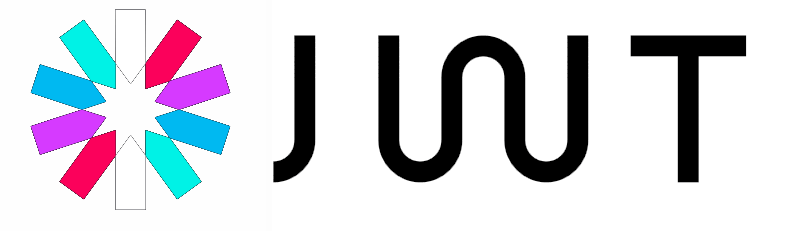
\includegraphics[scale=0.4]{ACR/jwt-logo.png}
        \caption{Logo JWT}
    \end{figure}

    JSON Web Token\cite{jwt} (\acs{JWT}) est une norme ouverte (RFC 7519) qui définit une méthode compacte et autonome pour la transmission sécurisée d'informations entre les parties (telles qu'un client et un serveur) en tant qu'objets JSON. Étant donné que ces informations sont signées numériquement, elles peuvent être vérifiées et fiables. \acs{JWT} peut être signé à l'aide d'un secret (à l'aide de l'algorithme HMAC) ou à l'aide d'une paire de clés publique/privée RSA ou ECDSA.\\
    
    \acs{JWT} est particulièrement populaire dans le processus d'authentification. Leurs messages courts peuvent être cryptés et peuvent indiquer en toute sécurité qui est l'expéditeur et s'il dispose des droits d'accès nécessaires. L'utilisateur lui-même n'a pas de contact indirect avec le token, par exemple lorsqu'il saisit le nom d'utilisateur et le mot de passe dans le masque. La vraie communication a lieu entre le client et le serveur.\\

    \subsection{Material UI}
    \begin{figure}[H]
        \centering
        
\includegraphics[scale=0.4]{ACR/materialui-logo.png}
        \caption{Logo Material UI}
    \end{figure}

    Material UI\cite{mui} est l'un des frameworks d'interface utilisateur React des plus reconnu. Il nous fournit des composants React qui implémentent Google Material Design. Material-UI a commencé avec l'implémentation React de la spécification Google Material Design en 2014.\\

    Material UI contiens plusieurs composants prêt a l'emploi et donne, donc, aux développeurs une très grande rapidité lors de la création des interfaces. Il est aussi très facile à personnaliser ce qui fait de lui l'un des frameworks les plus utilisés quand il s de création d'interfaces utiliser.\\

\section{Présentation des outils utilisés}
    \subsection{Visual Studio Code}
    \begin{figure}[H]
        \centering
        
\includegraphics[scale=0.1]{ACR/vscode-logo.png}
        \caption{Logo Visual Studio Code}
    \end{figure}

    Visual Studio Code\cite{vscode} est un éditeur de code source qui peut être utilisé dans plusieurs langages de programmation. Il est basé sur le framework Electron et est utilisé pour développer des applications Web Node.js s'exécutant sur le moteur de mise en page Blink.\\
    
    Visual Studio Code peut être étendu via des extensions, ce qui le rend très versatile, qui sont disponibles via un dépôt central. Cela inclut l'ajout d'un éditeur et la prise en charge des langues. Une caractéristique notable est la possibilité de créer des extensions pour ajouter la prise en charge de nouveaux langages, thèmes et débogueurs, d'effectuer une analyse de code statique.\\
    
    Dans l'enquête auprès des développeurs Stack Overflow de 2021, Visual Studio Code a été classé comme l'outil d'environnement de développement le plus populaire.

    \subsection{Dbeaver}
    \begin{figure}[H]
        \centering
        
\includegraphics[scale=0.1]{ACR/DBeaver-Logo.png}
        \caption{Logo DBeaver}
    \end{figure}
    
    DBeaver\cite{dbeaver} est un outil de gestion de base de données graphique gratuit et open source pour les développeurs et les administrateurs de base de données. Prêt à l'emploi, DBeaver prend en charge plus de 80 bases de données.\\
    
    À l'aide de DBeaver, on a la possibilité de manipuler les données comme dans des feuilles de calcul ordinaires, créer des rapports d'analyse basés sur les enregistrements de différents magasins de données et exporter des informations dans un format approprié. Pour les utilisateurs avancés de bases de données, DBeaver recommande l'utilisation d'un éditeur SQL puissant, de fonctions de gestion étendues, de fonctions de migration de données et de schémas, de surveillance des sessions de connexion à la base de données, etc.\\
    
    DBeaver est un outil multiplateforme disponible pour Windows, Linux, Mac et Solaris.\\

    \subsection{Github}
    \begin{figure}[H]
        \centering
        \includegraphics[scale=0.4]{ACR/Github-Logo.png}
        \caption{Logo Github}
    \end{figure}

    GitHub\cite{github} est une plate-forme de gestion de versions et de collaboration open source pour les développeurs de logiciels. La solution GitHub livrée sous forme de logiciel à la demande (SaaS, Software as a Service) a été lancée en 2008.\\
    
    Il est basé sur Git, un système de gestion de code open source créé par Linus Torvalds pour accélérer le développement de logiciels. L'interface de GitHub est très conviviale, même les codeurs novices peuvent profiter de Git. Si vous n'avez pas GitHub, l'utilisation de Git nécessite généralement plus de connaissances techniques et d'utilisation de la ligne de commande.\\

    \subsection{Discord}
    \begin{figure}[H]
        \centering
        
\includegraphics[scale=0.09]{ACR/Discord-Logo.png}
        \caption{Logo Discord}
    \end{figure}
    
    Discord\cite{discord} est une plate-forme de chat et de messagerie en ligne conçue pour une utilisation en groupe. Comme il est réservé aux invités, il s'agit d'un espace sûr où les étudiants peuvent interagir sans avoir à rester ensemble dans la pièce. L'application de messagerie d'équipe se concentre principalement sur le chat vocal. L'option de chat textuel n'est pas aussi étendue que le canal vocal dans ses produits.\\

    Il s'agit d'un système très facile à utiliser et qui peut également être mis en place rapidement. Par conséquent, cela peut faciliter la transition vers l'enseignement à distance ou les classes hybrides, tout en créant l'impression que tout le monde est dans la même pièce. La vidéo et l'audio à faible latence permettent d'obtenir une réponse quasi instantanée, tout comme le chat dans le monde réel.\\

    \subsection{Draw.io}
    \begin{figure}[H]
        \centering
        
\includegraphics[scale=0.4]{ACR/Drawio-Logo.png}
        \caption{Logo Draw.io}
    \end{figure}

    Draw.io\cite{drawio} est conçu par Seibert Media et est un logiciel propriétaire permettant de créer des tableaux et des graphiques. Le logiciel vous permet de sélectionner des fonctions de mise en page automatiques ou de créer des mises en page personnalisées. Ils ont une variété de formes et des centaines d'éléments visuels parmi lesquels choisir, ce qui rend votre tableau ou graphique unique. La fonction glisser-déposer peut facilement créer des tableaux ou des graphiques attrayants.\\

    Par rapport à l'utilisation d'un logiciel vectoriel, cet outil peut vous aider à créer plus facilement des diagrammes et d'autres effets visuels. Lorsqu'il est utilisé avec Google Drive, Draw.io prend en charge la collaboration en temps réel afin que plusieurs personnes puissent travailler sur le graphique en même temps.\\

\section{Présentation des interfaces}
    Dans le contenu suivant, nous montrerons un aperçu du rendu final de notre application et quelle ques interfaces qui la composent.

    \subsection{Interface d'accueil}
    \begin{figure}[H]
        \centering
        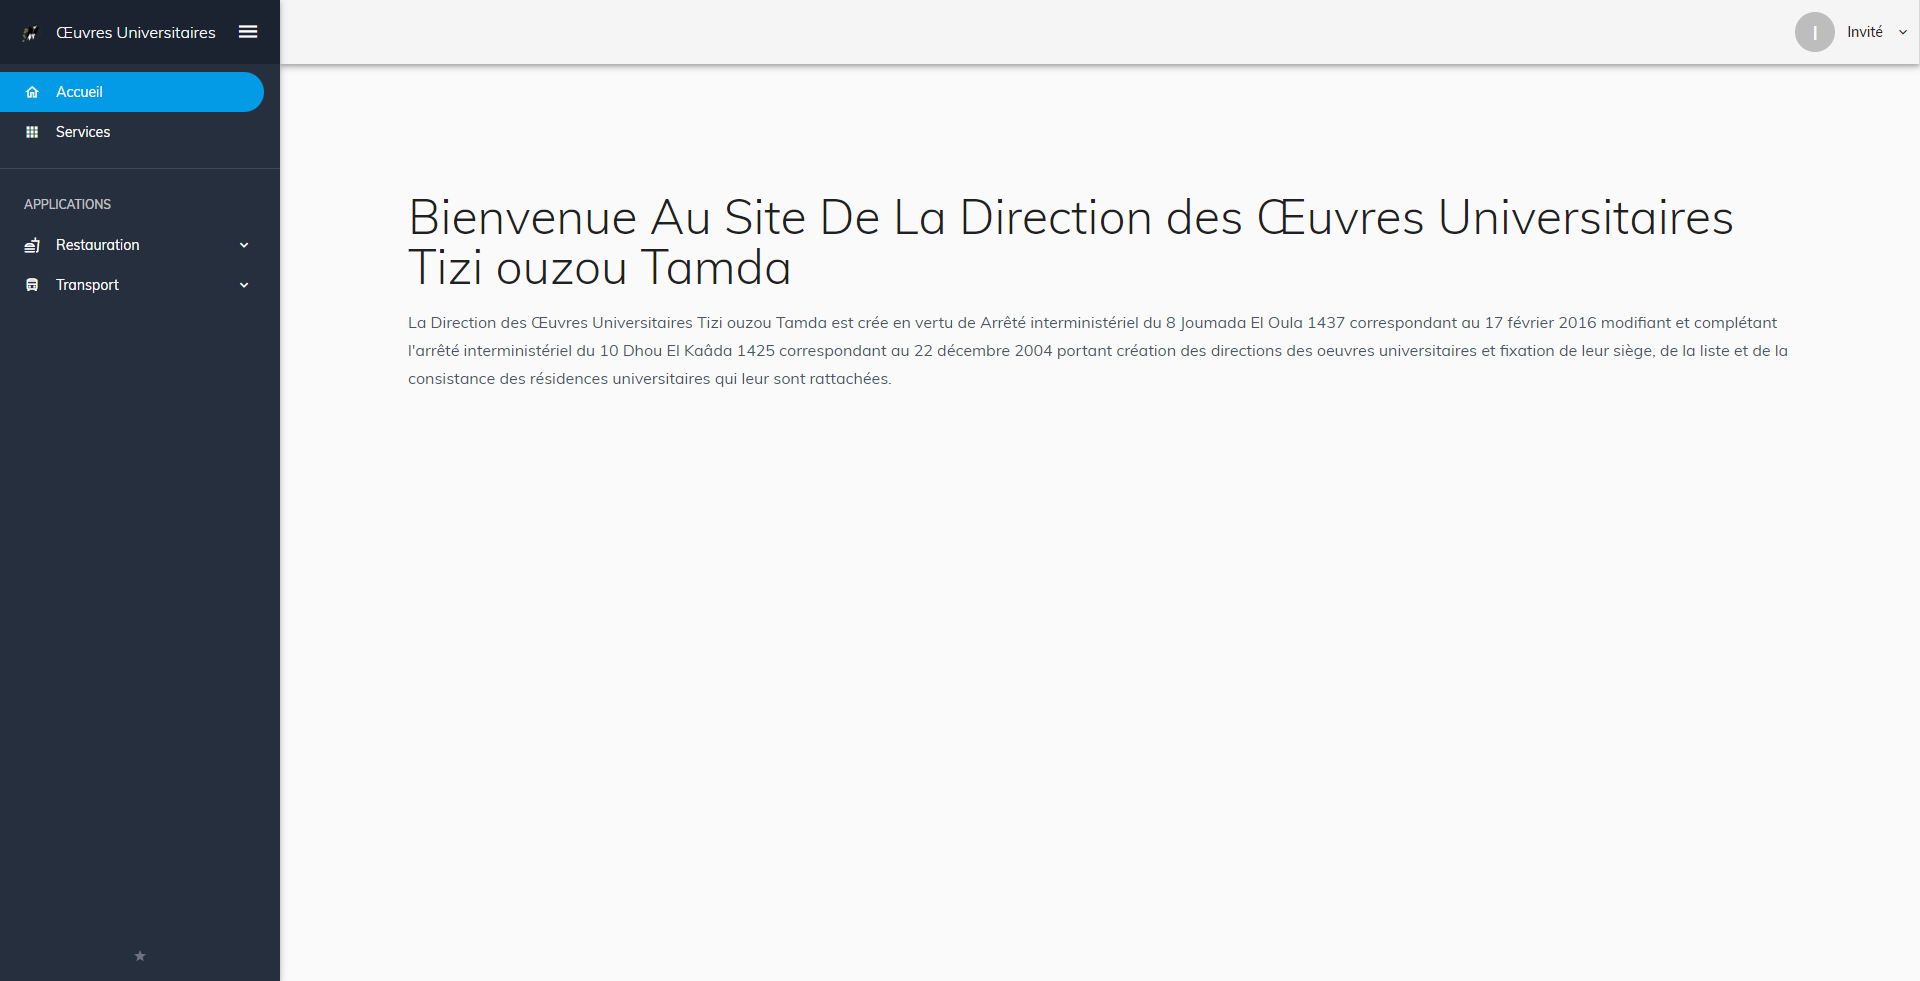
\includegraphics[scale=0.21]{PFE Screens/Invité/accueil.jpg}
        \caption{Interface d'accueil}
    \end{figure}

    \subsection{Interface d'authentification}
    \begin{figure}[H]
        \centering
        
\includegraphics[scale=0.21]{PFE Screens/Connection.jpg}
        \caption{Interface d'authentification}
    \end{figure}

    \subsection{Interface invité 'Services'}
    \begin{figure}[H]
        \centering
        \includegraphics[scale=0.21]{PFE Screens/Invité/Services.jpg}
        \caption{Interface invité 'Services'}
    \end{figure}

    \subsection{Interface invité 'Calendrier des menus'}
    \begin{figure}[H]
        \centering
        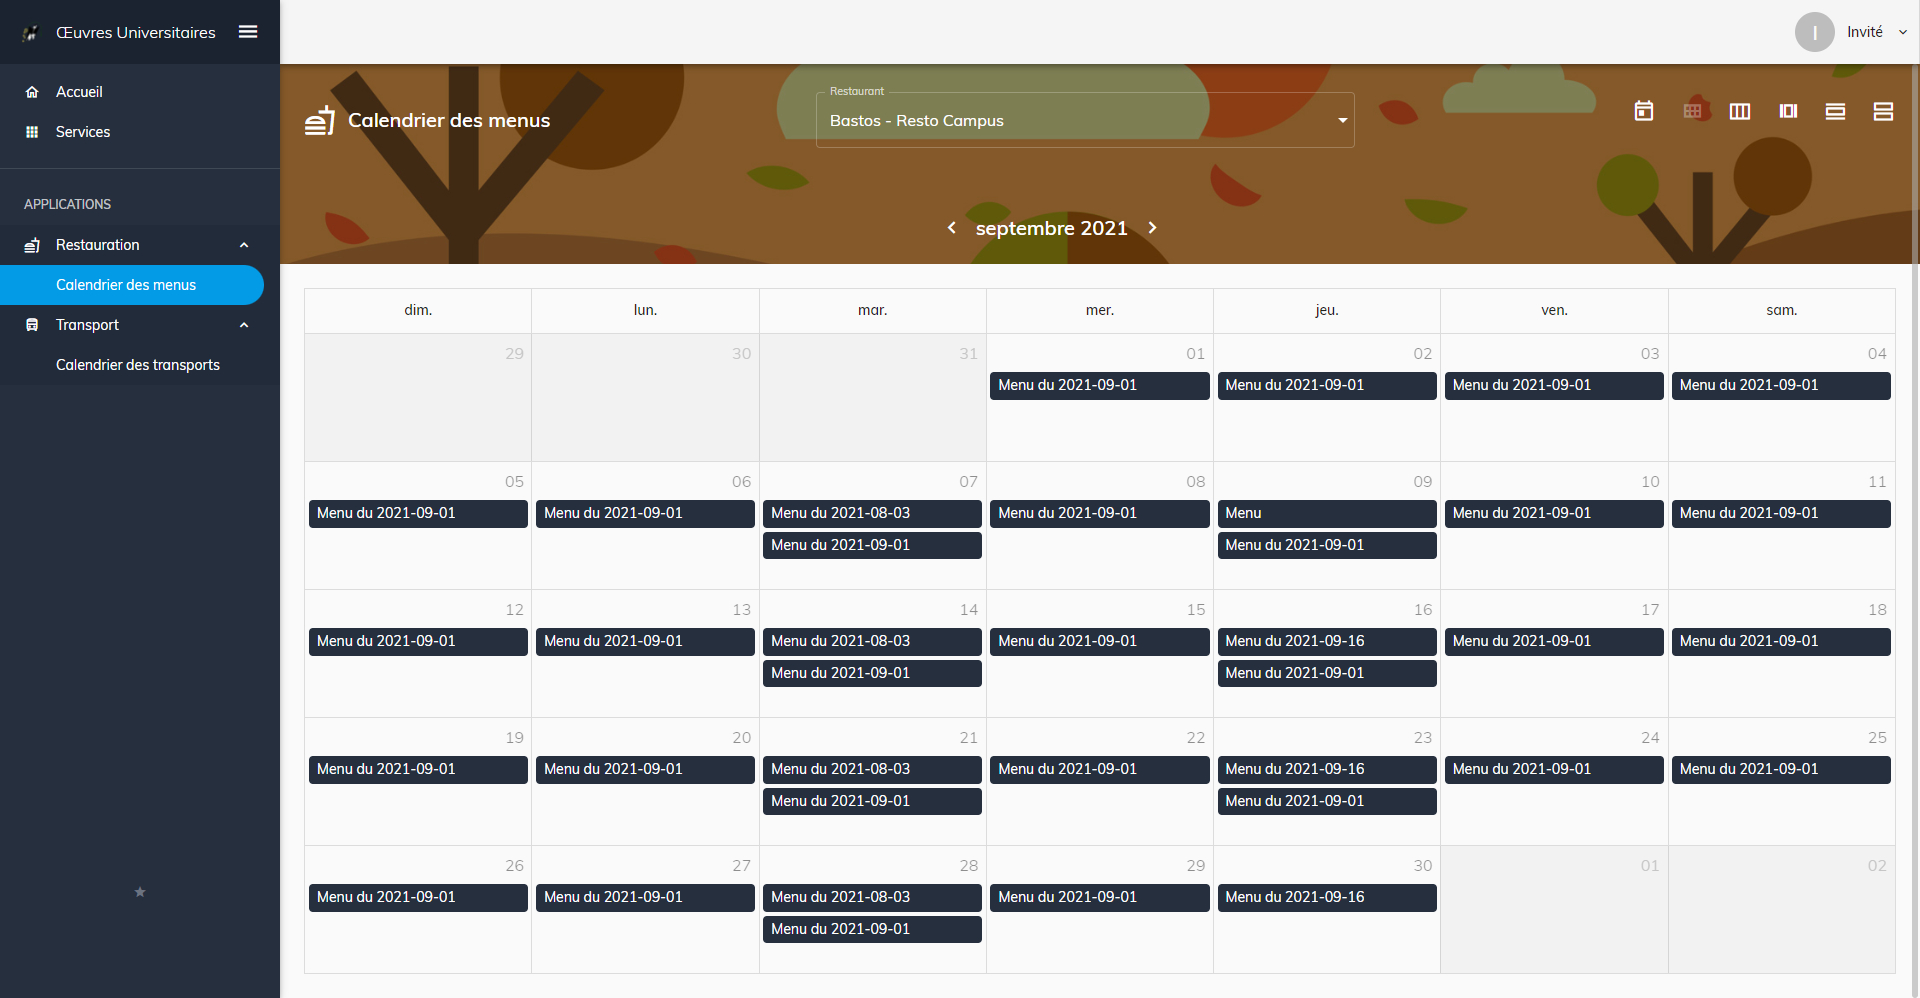
\includegraphics[scale=0.21]{PFE Screens/Invité/Restauration/Calendrier des menus.jpg}
        \caption{Interface invité 'Calendrier des menus'}
    \end{figure}

    \subsection{Interface invité 'Détail d'un menus'}
    \begin{figure}[H]
        \centering
        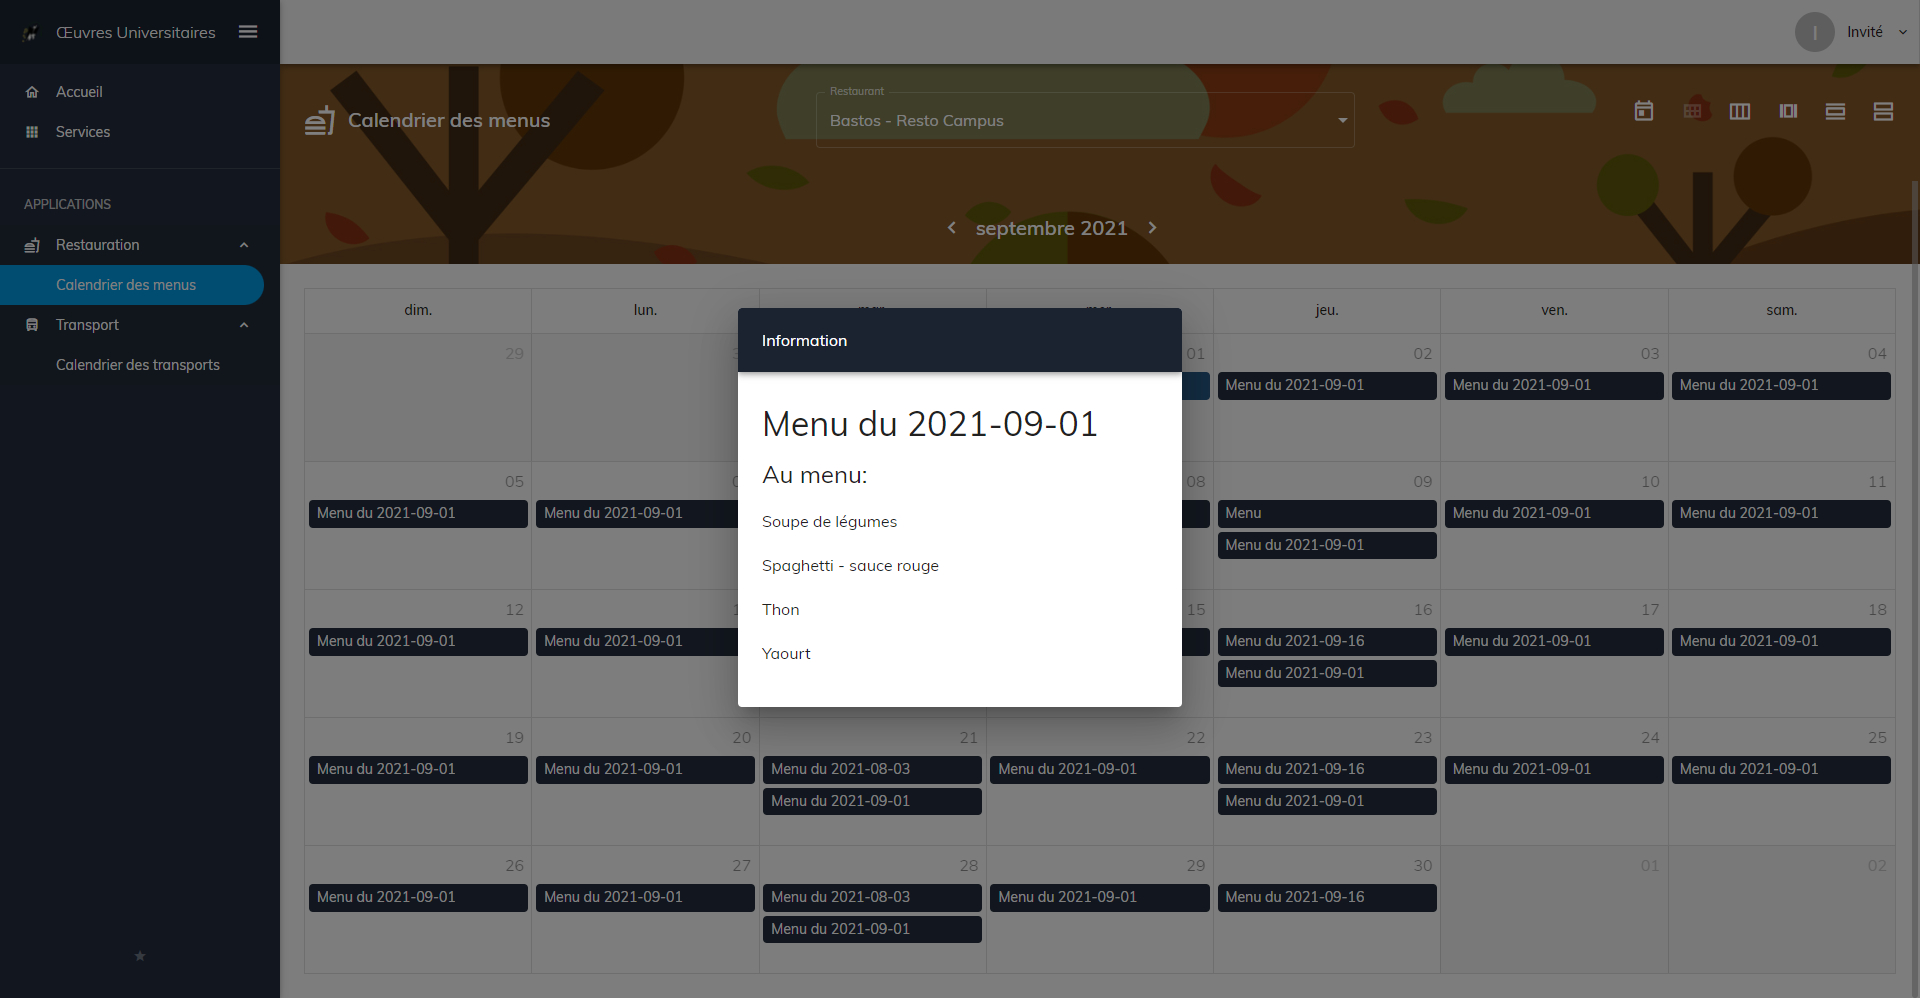
\includegraphics[scale=0.21]{PFE Screens/Invité/Restauration/Calendrier des menus - Détail.jpg}
        \caption{Interface invité 'Détail d'un menus'}
    \end{figure}
    
    \subsection{Interface d'accueil utilisateur}
    \begin{figure}[H]
        \centering
        
\includegraphics[scale=0.21]{PFE Screens/Admin/Accueil.jpg}
        \caption{Interface d'accueil utilisateur}
    \end{figure}

    \subsection{Interface utilisateur utilisateur 'Dossiers d'hebergements'}
    \begin{figure}[H]
        \centering
        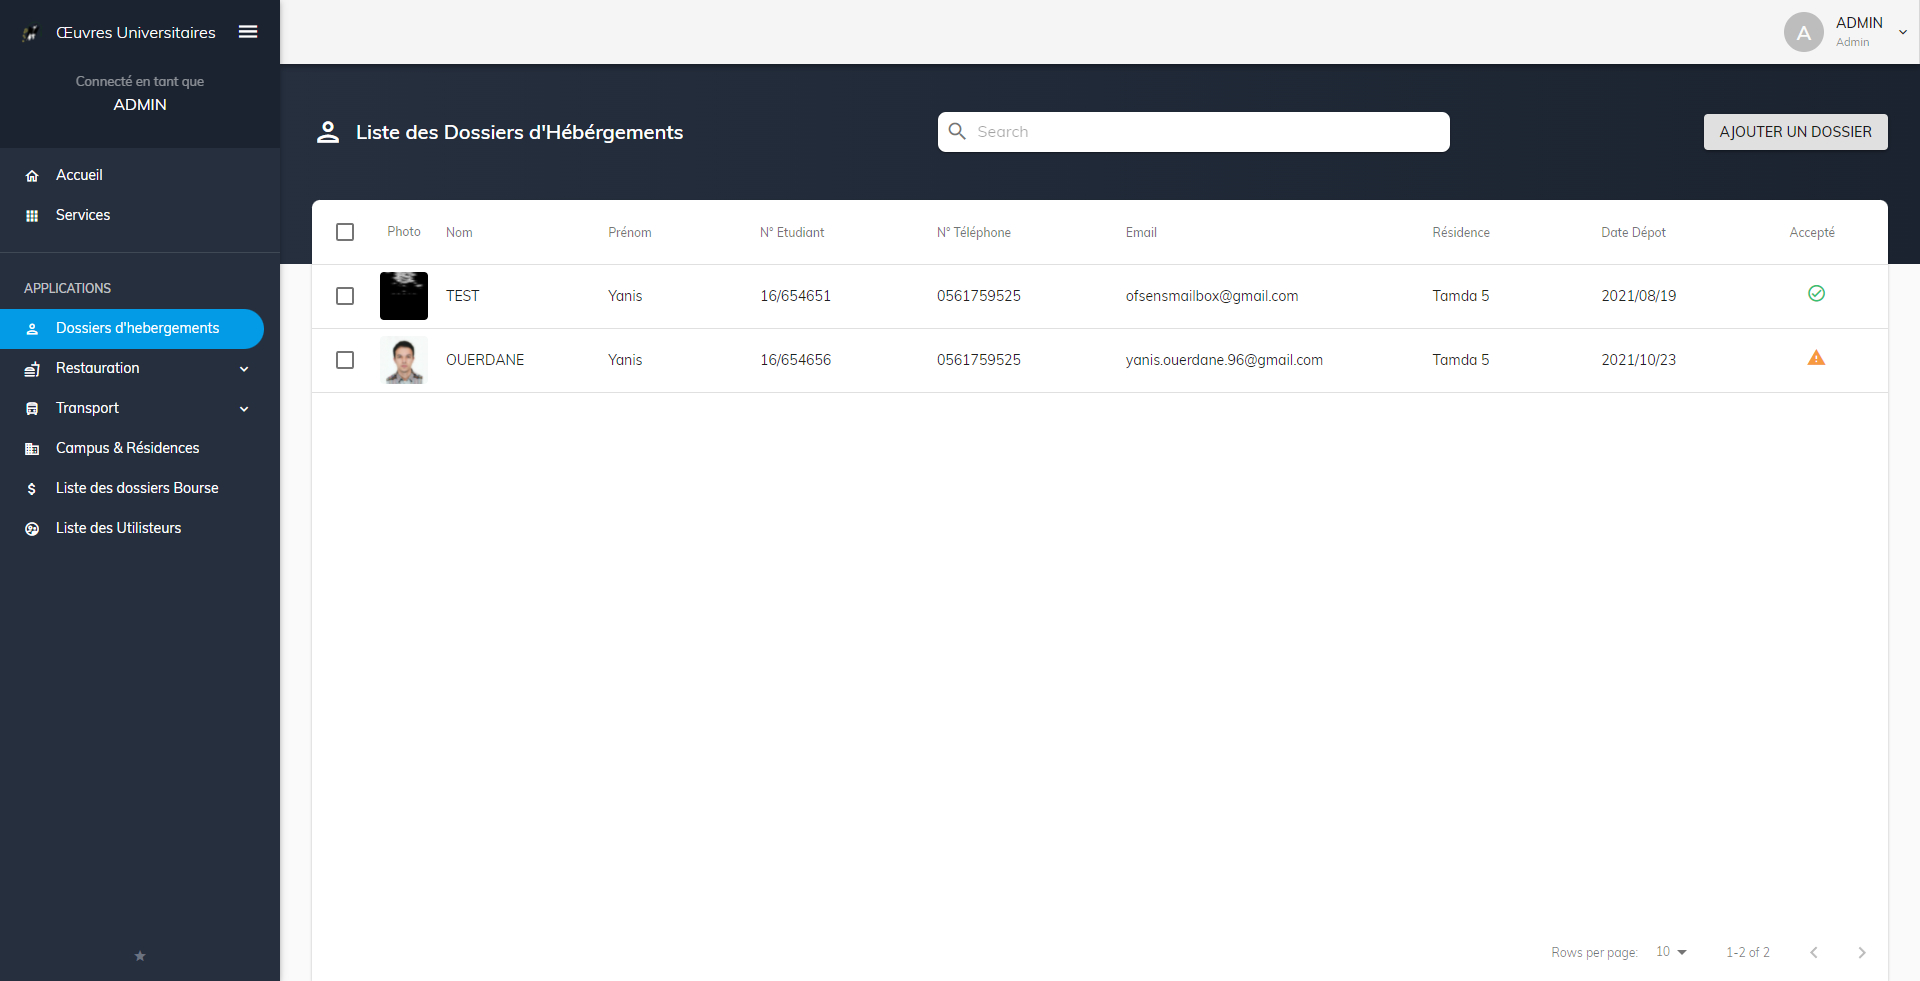
\includegraphics[scale=0.21]{PFE Screens/Admin/Hebergement/Liste des Dossiers d'Hébérgements.jpg}
        \caption{Interface utilisateur 'Dossiers d'hebergements'}
    \end{figure}

    \subsection{Interface utilisateur détail d'un dossier d'hebergements}
    \begin{figure}[H]
        \centering
        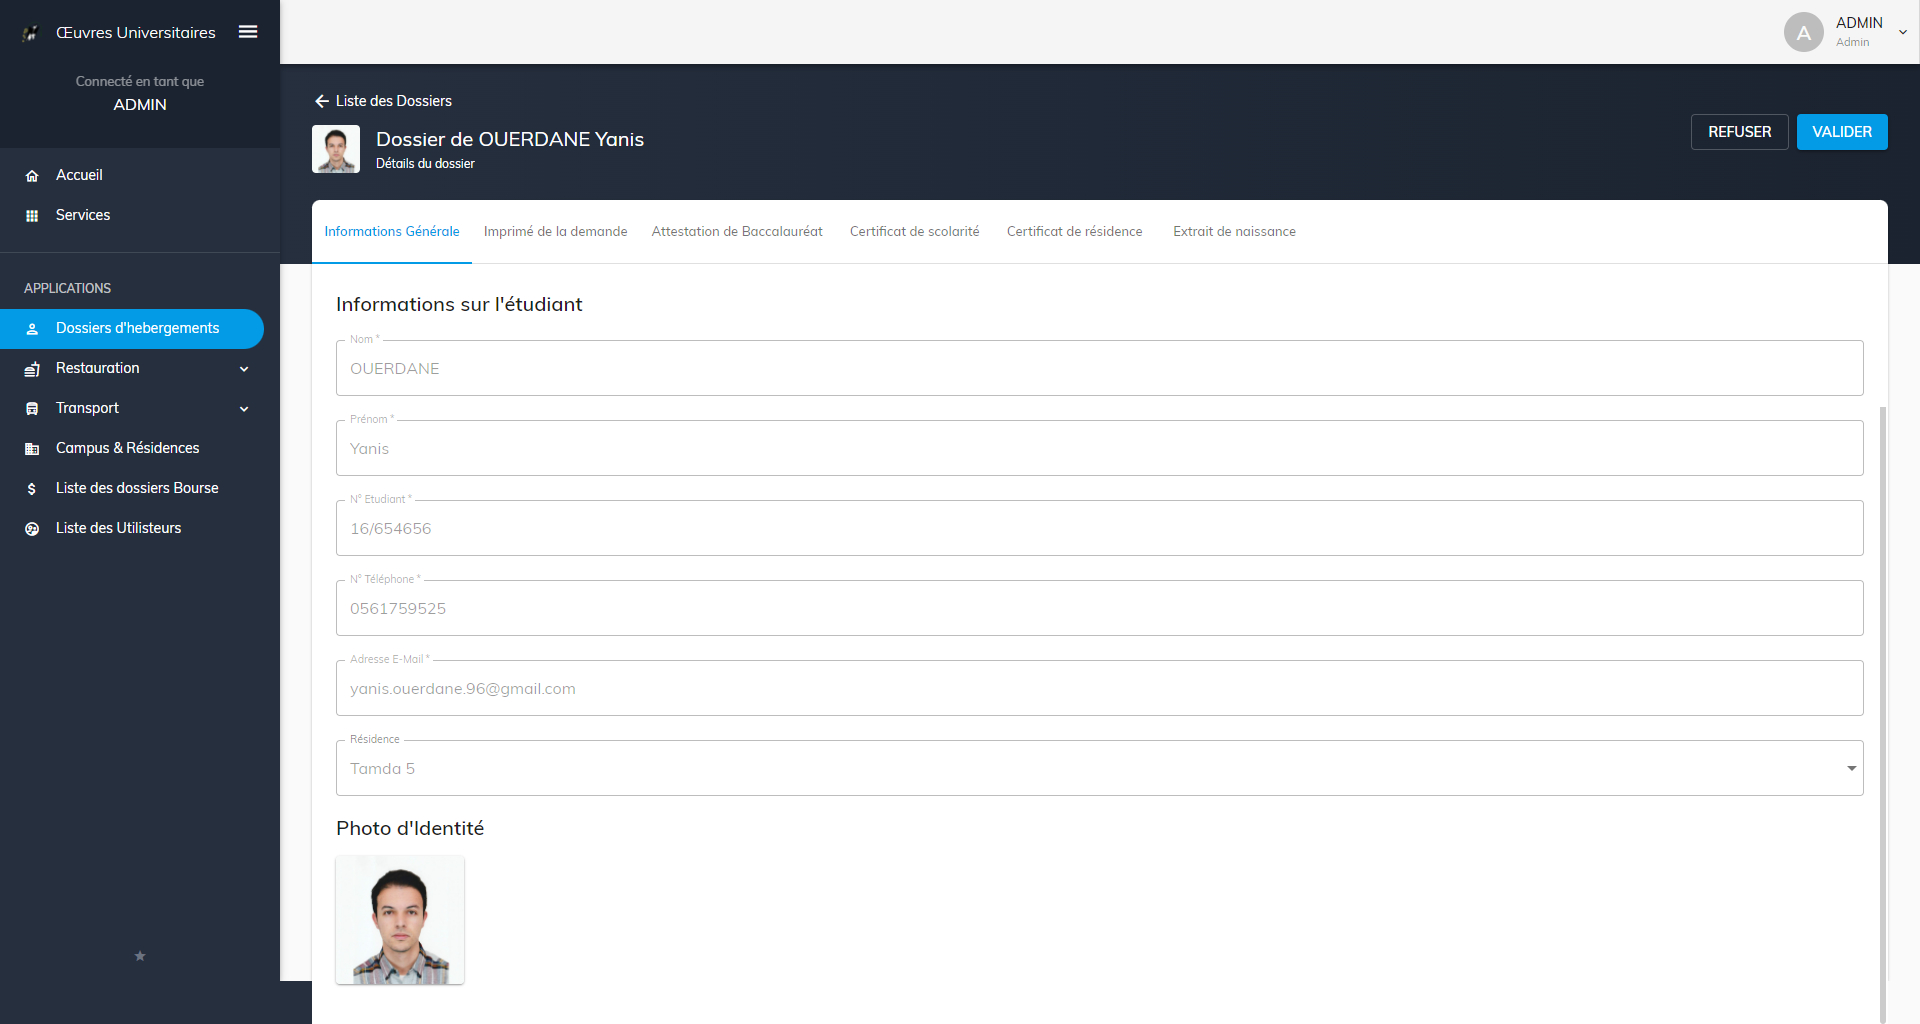
\includegraphics[scale=0.21]{PFE Screens/Admin/Hebergement/Detail.jpg}
        \caption{Interface utilisateur détail d'un dossier d'hebergements}
    \end{figure}

    \subsection{Interface utilisateur 'Liste des Réstaurants'}
    \begin{figure}[H]
        \centering
        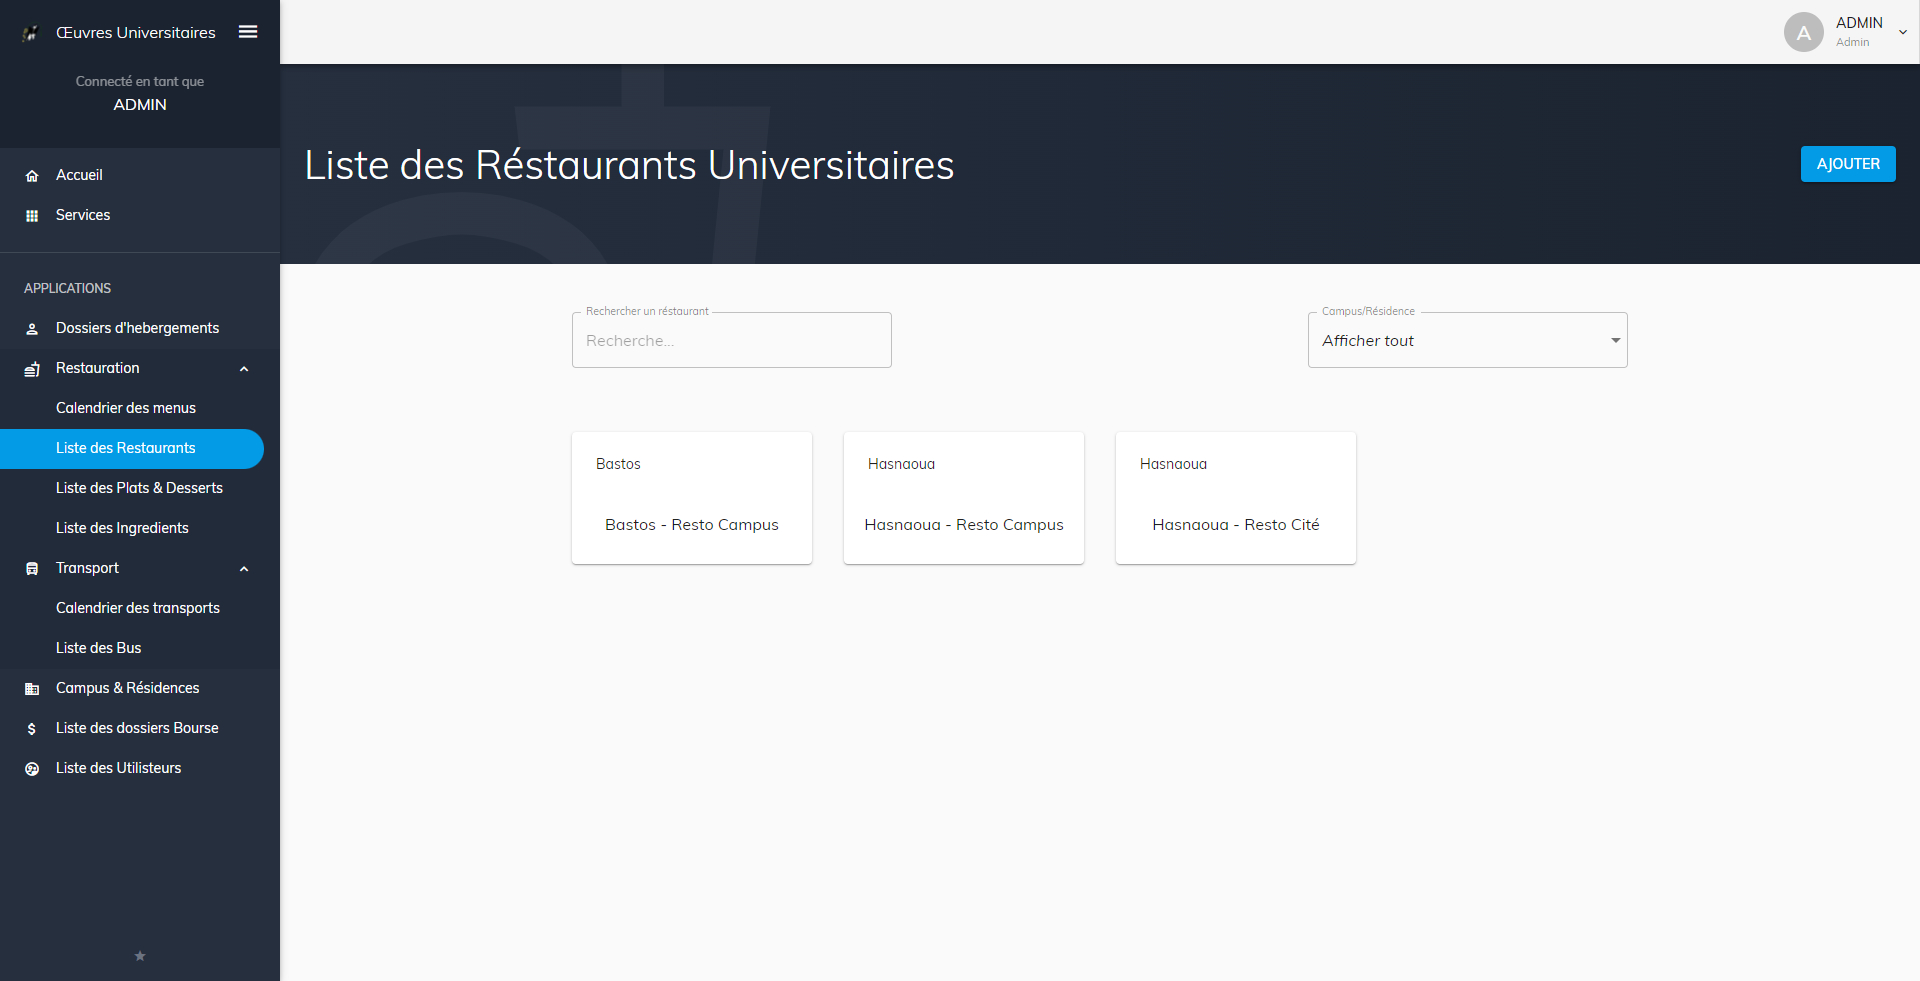
\includegraphics[scale=0.21]{PFE Screens/Admin/Restauration/Restos/Restos.jpg}
        \caption{Interface utilisateur 'Liste des Réstaurants'}
    \end{figure}

    \subsection{Interface utilisateur 'Modifier un réstaurant'}
    \begin{figure}[H]
        \centering
        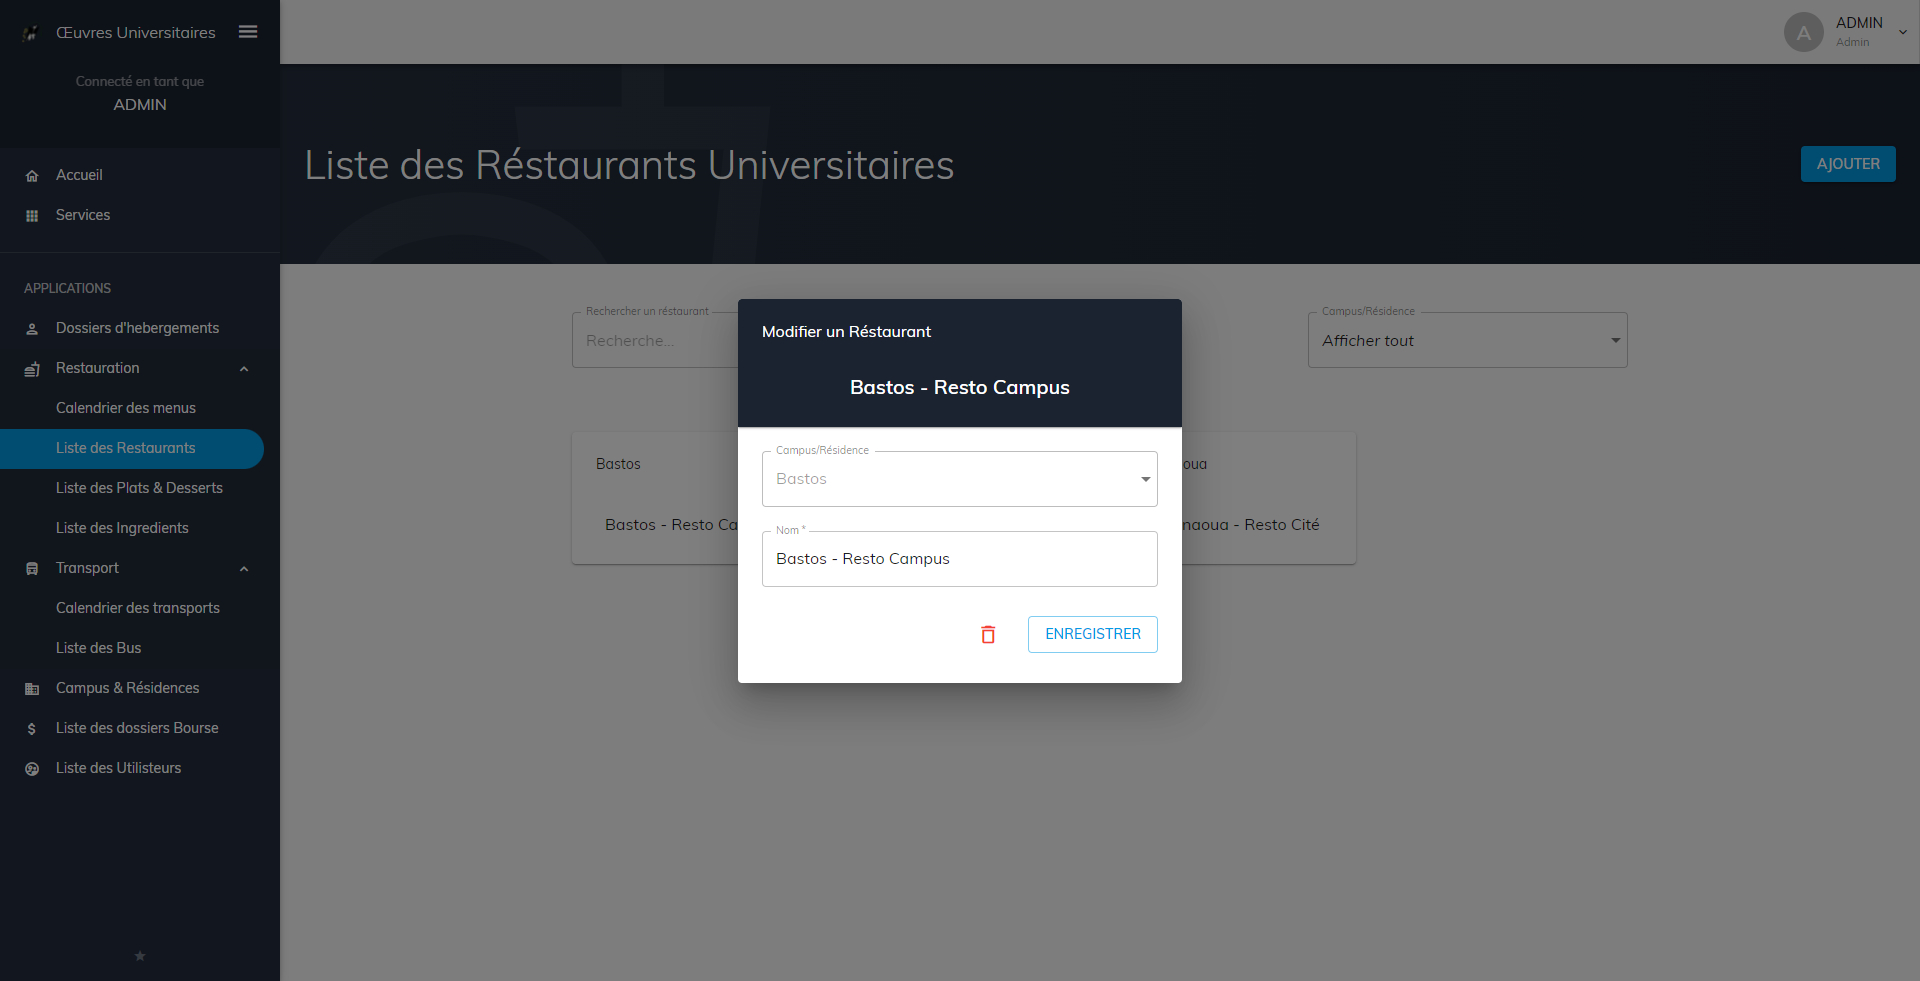
\includegraphics[scale=0.21]{PFE Screens/Admin/Restauration/Restos/Modif - Resto.jpg}
        \caption{Interface utilisateur 'Modifier un réstaurant'}
    \end{figure}

    \subsection{Interface utilisateur 'Liste des Ingredients'}
    \begin{figure}[H]
        \centering
        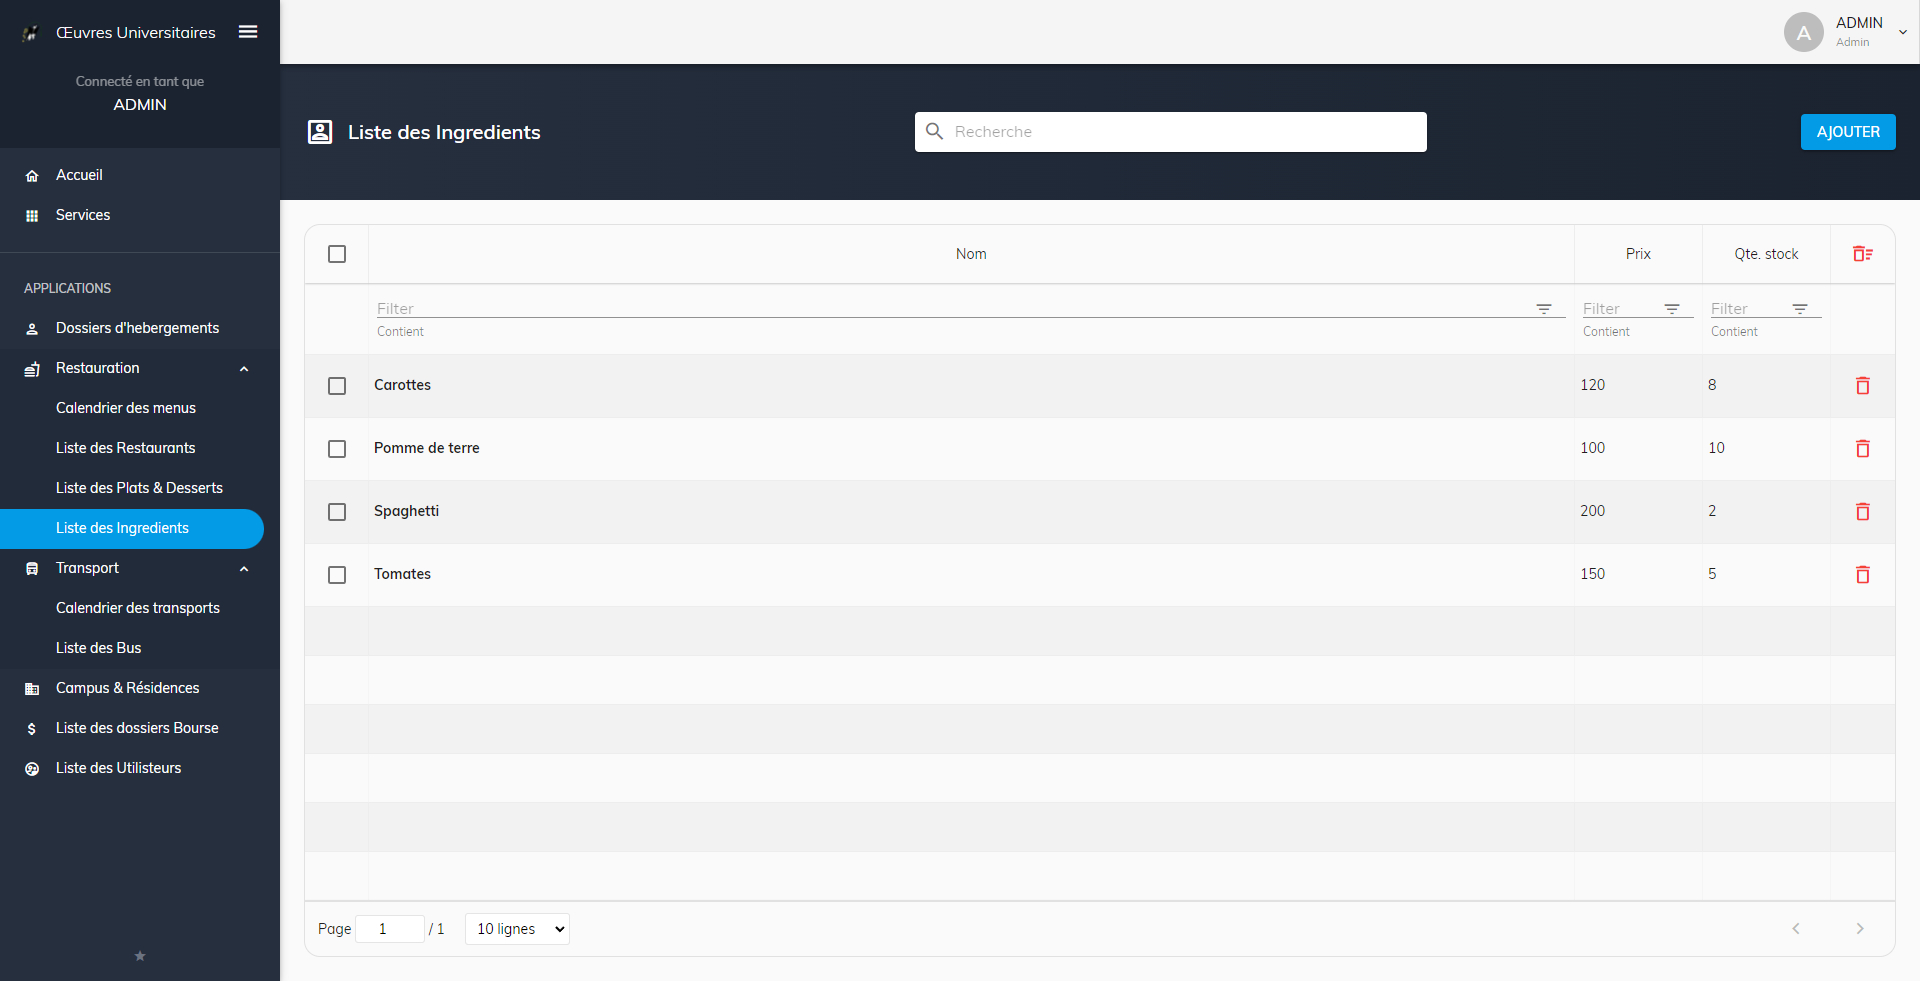
\includegraphics[scale=0.21]{PFE Screens/Admin/Restauration/Ingredients/liste.jpg}
        \caption{Interface utilisateur 'Liste des Ingredients'}
    \end{figure}
    
    \subsection{Interface utilisateur - Détails des menus du mois}
    \begin{figure}[H]
        \centering
        \includegraphics[scale=0.21]{PFE Screens/Admin/Restauration/Calendrier/Détails du moi.jpg}
        \caption{Interface utilisateur - Détails des menus du mois}
    \end{figure}

\section{Conclusion}
Dans ce chapitre nous avons montré l'environnement de travail, les outils utiliser pour créer notre application ainsi que les techniques et les bibliothèques qui nous ont aider dans ce processus.\\

Par la suite, nous avons présenté quelles ques interfaces du rendu final de notre application.\\

Tout en respectant le concept développé lors de l'analyse, nous avons pu réaliser les objectifs fixés.\\